% ============================================================================
% CHAPTER 1A: MODELING FUNDAMENTALS
% ============================================================================

% \chapter{System Modeling with Ideal Components}
\label{ch:modeling}

\begin{keyconceptbox}[title=Learning Objectives]
After completing this chapter, you will be able to:
\begin{itemize}
    \item Understand the purpose and process of mathematical modeling
    \item Apply ideal sensor and actuator assumptions appropriately
    \item Derive differential equations from physical principles
    \item Convert between different model representations
    \item Recognize analogies between different physical domains
\end{itemize}
\end{keyconceptbox}

The foundation of control systems engineering is the mathematical model---a set of equations that describe how a system behaves. Before we can analyze stability, design controllers, or implement feedback, we must first capture the essential dynamics of the system we wish to control.

This chapter introduces systematic approaches to modeling physical systems across diverse engineering domains. We begin with ideal assumptions: perfect sensors that measure exactly what we want, and ideal actuators that respond instantly with unlimited capability. These assumptions let us focus on the fundamental physics before adding real-world complications in later chapters.

% ============================================================================
\chapter{The Art and Science of Modeling}
\label{ch:modeling_philosophy}
% ============================================================================

\section{Why Model?}

Mathematical models serve several critical purposes in control engineering:

\begin{enumerate}
    \item \textbf{Prediction}: Models let us simulate system behavior before building hardware, saving time and money.

    \item \textbf{Analysis}: We can mathematically determine stability, performance limits, and sensitivities.

    \item \textbf{Design}: Controllers are designed based on models---better models lead to better controllers.

    \item \textbf{Understanding}: The modeling process itself reveals what physical parameters matter most.
\end{enumerate}

\begin{quote}
\textit{``All models are wrong, but some are useful.''} --- George E.P. Box
\end{quote}

A model is always an approximation. The goal is not perfect fidelity but rather capturing the dynamics relevant to control at the frequencies and amplitudes of interest.

\begin{historicalbox}[title=Historical Context: Watt's Flyball Governor and Early Feedback Control]
The first automatic feedback controller was James Watt's flyball governor (1788), a mechanical device that regulated the speed of steam engines by adjusting fuel flow based on centrifugal force from rotating weights. When engine speed increased, the weights flew outward, reducing fuel flow; when speed decreased, they fell inward, increasing flow. This elegant mechanical feedback system enabled the Industrial Revolution by allowing steam engines to operate autonomously without constant human adjustment. Remarkably, no mathematical model existed for analyzing this system's stability---early engineers relied on trial-and-error design.

The mathematical analysis of feedback control began over 80 years later when James Clerk Maxwell, famous for electromagnetism, published a seminal paper in 1868 analyzing the stability of the flyball governor using differential equations. Maxwell showed that the governor's stability depended on system parameters and introduced the concept that a feedback system could become unstable if parameters were chosen incorrectly. His 1868 paper laid the mathematical foundation for all subsequent control theory, proving that governing equations could predict whether a system would oscillate or diverge---a revolutionary insight that transformed control from an art into a science.
\end{historicalbox}

\section{The Modeling Process}

\begin{figure}[htbp]
\centering
\begin{tikzpicture}[node distance=2cm, auto,
    block/.style={rectangle, draw, text width=3cm, text centered, minimum height=1cm},
    arrow/.style={->, >=stealth, thick}]

    \node[block] (physical) {Physical System};
    \node[block, right=of physical] (assumptions) {Assumptions \& Simplifications};
    \node[block, right=of assumptions] (equations) {Governing Equations};
    \node[block, below=of equations] (model) {Mathematical Model};
    \node[block, left=of model] (validate) {Validation \& Refinement};
    \node[block, left=of validate] (apply) {Apply to Control Design};

    \draw[arrow] (physical) -- (assumptions);
    \draw[arrow] (assumptions) -- (equations);
    \draw[arrow] (equations) -- (model);
    \draw[arrow] (model) -- (validate);
    \draw[arrow] (validate) -- (apply);
    \draw[arrow, dashed] (validate) |- ++(0,1.5) -| (assumptions);
\end{tikzpicture}
\caption{The iterative modeling process.}
\label{fig:modeling_process}
\end{figure}


The modeling process typically involves:

\begin{enumerate}
    \item \textbf{Define the system boundary}: What is included? What is external?

    \item \textbf{Identify inputs and outputs}: What can we manipulate? What do we measure?

    \item \textbf{List assumptions}: What simplifications are appropriate?

    \item \textbf{Apply physical laws}: Conservation of energy, mass, momentum, charge, etc.

    \item \textbf{Derive equations}: Combine physical laws into mathematical form.

    \item \textbf{Validate}: Compare model predictions with experimental data.

    \item \textbf{Refine}: Add complexity only where needed.
\end{enumerate}

% ============================================================================
\chapter{Ideal Assumptions}
\label{ch:ideal_assumptions}
% ============================================================================

Throughout this chapter, we make two fundamental idealizations:

\section{Ideal Sensors}

An \textbf{ideal sensor} provides a perfect measurement of the quantity of interest:

\begin{itemize}
    \item \textbf{No delay}: The measurement is instantaneous
    \item \textbf{No noise}: The measurement has no random errors
    \item \textbf{No bias}: The measurement has no systematic offset
    \item \textbf{Infinite bandwidth}: All frequencies are captured equally
    \item \textbf{Infinite resolution}: Any value can be measured exactly
    \item \textbf{No loading}: The sensor does not affect the measured quantity
\end{itemize}

Mathematically, if $x(t)$ is the true value, the ideal sensor output is:
\begin{equation}
y_{\text{measured}}(t) = x(t)
\end{equation}

\section{Ideal Actuators}

An \textbf{ideal actuator} produces exactly the commanded output:

\begin{itemize}
    \item \textbf{No delay}: Response is instantaneous
    \item \textbf{No dynamics}: No transient behavior in the actuator itself
    \item \textbf{Infinite bandwidth}: Can track any commanded signal perfectly
    \item \textbf{Unlimited force/torque/power}: No saturation limits
    \item \textbf{Infinite acceleration}: Can change output instantly
    \item \textbf{No backlash or friction}: Perfect mechanical transmission
\end{itemize}

Mathematically, if $u(t)$ is the commanded input, the ideal actuator produces:
\begin{equation}
F_{\text{actual}}(t) = u(t) \quad \text{(or voltage, torque, flow rate, etc.)}
\end{equation}

\begin{warningbox}
Real sensors and actuators violate all of these assumptions to varying degrees. Chapters on sensor modeling and actuator dynamics will address these non-idealities. For now, ideal assumptions let us focus on the plant dynamics.
\end{warningbox}

% ============================================================================
\chapter{Fundamental Physical Laws}
\label{ch:physical_laws}
% ============================================================================

Most dynamic systems can be modeled using a small set of conservation principles:

\section{Newton's Laws (Mechanical)}

\textbf{Newton's Second Law} for translation:
\begin{equation}
\sum F = ma = m\frac{\dd^2 x}{\dd t^2}
\end{equation}

\textbf{Rotational analog}:
\begin{equation}
\sum \tau = J\alpha = J\frac{\dd^2 \theta}{\dd t^2}
\end{equation}

where $J$ is the moment of inertia and $\alpha$ is angular acceleration.

\section{Kirchhoff's Laws (Electrical)}

\textbf{Kirchhoff's Voltage Law (KVL)}: The sum of voltages around any closed loop is zero:
\begin{equation}
\sum_{\text{loop}} V = 0
\end{equation}

\textbf{Kirchhoff's Current Law (KCL)}: The sum of currents at any node is zero:
\begin{equation}
\sum_{\text{node}} i = 0
\end{equation}

\section{Conservation of Energy (Thermal)}

\begin{equation}
\frac{\dd E}{\dd t} = \dot{Q}_{\text{in}} - \dot{Q}_{\text{out}} + \dot{W}
\end{equation}

For thermal systems:
\begin{equation}
mC_p\frac{\dd T}{\dd t} = \dot{Q}_{\text{in}} - \dot{Q}_{\text{out}}
\end{equation}

\section{Conservation of Mass (Fluid/Chemical)}

\begin{equation}
\frac{\dd m}{\dd t} = \dot{m}_{\text{in}} - \dot{m}_{\text{out}}
\end{equation}

For incompressible fluids with density $\rho$ and volume $V$:
\begin{equation}
\rho\frac{\dd V}{\dd t} = \rho Q_{\text{in}} - \rho Q_{\text{out}}
\end{equation}

where $Q$ is volumetric flow rate.

% ============================================================================
\chapter{Model Representations}
\label{ch:model_representations}
% ============================================================================

The same dynamic system can be represented in several equivalent forms:

\section{Differential Equation Form}

The most direct form, derived from physical laws:
\begin{equation}
a_n\frac{\dd^n y}{\dd t^n} + a_{n-1}\frac{\dd^{n-1} y}{\dd t^{n-1}} + \cdots + a_1\frac{\dd y}{\dd t} + a_0 y = b_m\frac{\dd^m u}{\dd t^m} + \cdots + b_0 u
\end{equation}

\section{Transfer Function Form}

Taking the Laplace transform (with zero initial conditions):
\begin{equation}
G(s) = \frac{Y(s)}{U(s)} = \frac{b_m s^m + b_{m-1}s^{m-1} + \cdots + b_0}{a_n s^n + a_{n-1}s^{n-1} + \cdots + a_0}
\end{equation}

\section{State-Space Form}

\begin{align}
\dot{\vecx} &= \mA\vecx + \mB\vecu \\
\vecy &= \mC\vecx + \mD\vecu
\end{align}

where $\vecx$ is the state vector containing the minimum information needed to predict future behavior.

\section{Block Diagram Form}

A graphical representation showing signal flow and interconnections.

\begin{figure}[htbp]
\centering
\begin{tikzpicture}[auto, node distance=2cm]
    \node[input] (input) {};
    \node[block, right=of input] (G) {$G(s)$};
    \node[output, right=of G] (output) {};

    \draw[->] (input) -- node {$U(s)$} (G);
    \draw[->] (G) -- node {$Y(s)$} (output);
\end{tikzpicture}
\caption{Simple block diagram representation.}
\label{fig:simple_block}
\end{figure}


% ============================================================================
\chapter{System Analogies}
\label{ch:analogies}
% ============================================================================

Remarkably, systems from different physical domains often share the same mathematical structure. This allows us to transfer intuition and analysis techniques across domains.

\begin{table}[htbp]
\centering
\begin{tabular}{llll}
\toprule
\textbf{Concept} & \textbf{Mechanical (Trans.)} & \textbf{Electrical} & \textbf{Thermal} \\
\midrule
Effort (across) & Force $F$ & Voltage $V$ & Temperature $T$ \\
Flow (through) & Velocity $v$ & Current $i$ & Heat flow $\dot{Q}$ \\
Resistance & Damper $b$ & Resistor $R$ & Thermal res. $R_t$ \\
Capacitance & Spring $1/k$ & Capacitor $C$ & Thermal cap. $C_t$ \\
Inductance & Mass $m$ & Inductor $L$ & --- \\
\bottomrule
\end{tabular}
\caption{Analogous quantities across physical domains (force-voltage analogy).}
\label{tab:analogies}
\end{table}

\begin{examplebox}[title=Example 1.1: Mass-Spring-Damper $\equiv$ RLC Circuit]
The mechanical system:
\begin{equation}
m\ddot{x} + b\dot{x} + kx = F(t)
\end{equation}

is mathematically identical to the series RLC circuit:
\begin{equation}
L\ddot{q} + R\dot{q} + \frac{1}{C}q = V(t)
\end{equation}

Both have the same transfer function form:
\begin{equation}
G(s) = \frac{1}{ms^2 + bs + k} \equiv \frac{1}{Ls^2 + Rs + 1/C}
\end{equation}
\end{examplebox}

% ============================================================================
\chapter{Standard Test Inputs}
\label{ch:test_inputs}
% ============================================================================

To characterize system behavior, we use standard test inputs:

\section{Impulse Input}

\begin{equation}
u(t) = \delta(t), \quad U(s) = 1
\end{equation}

The impulse response $h(t) = \iLaplace\{G(s)\}$ completely characterizes an LTI system.

\section{Step Input}

\begin{equation}
u(t) = A \cdot \unitstep, \quad U(s) = \frac{A}{s}
\end{equation}

Step response reveals settling time, overshoot, and steady-state error.

\section{Ramp Input}

\begin{equation}
u(t) = At \cdot \unitstep, \quad U(s) = \frac{A}{s^2}
\end{equation}

Ramp response reveals tracking ability for constantly changing references.

\section{Sinusoidal Input}

\begin{equation}
u(t) = A\sin(\omega t), \quad U(s) = \frac{A\omega}{s^2 + \omega^2}
\end{equation}

Sinusoidal response at various frequencies reveals the frequency response.

\begin{figure}[htbp]
\centering
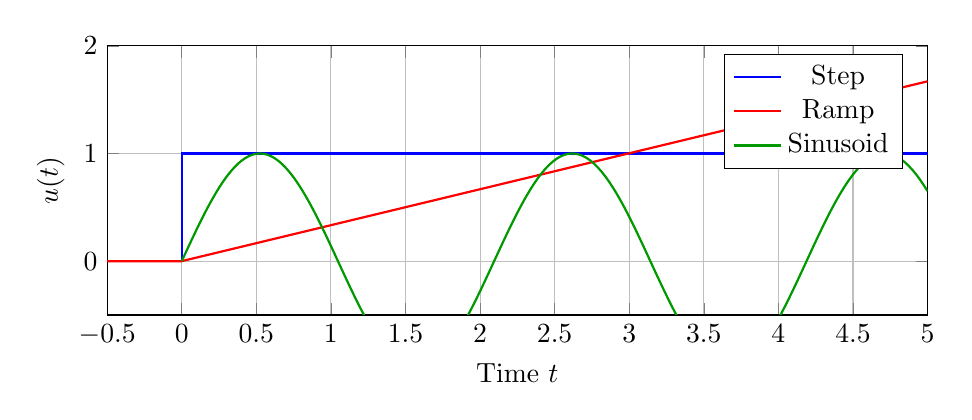
\begin{tikzpicture}
\begin{axis}[
    width=12cm, height=5cm,
    xlabel={Time $t$},
    ylabel={$u(t)$},
    xmin=-0.5, xmax=5,
    ymin=-0.5, ymax=2,
    legend pos=north east,
    grid=major,
    domain=0:5,
    samples=200
]
\addplot[blue, thick] coordinates {(-0.5,0) (0,0) (0,1) (5,1)};
\addlegendentry{Step}

\addplot[red, thick] coordinates {(-0.5,0) (0,0) (5,1.67)};
\addlegendentry{Ramp}

\addplot[green!60!black, thick] {sin(deg(3*x))};
\addlegendentry{Sinusoid}
\end{axis}
\end{tikzpicture}
\caption{Standard test inputs for system characterization.}
\label{fig:test_inputs}
\end{figure}


% ============================================================================
\chapter{First and Second Order System Responses}
\label{ch:standard_responses}
% ============================================================================

\section{First-Order Systems}

The standard first-order transfer function:
\begin{equation}
G(s) = \frac{K}{\tau s + 1}
\end{equation}

where:
\begin{itemize}
    \item $K$ = DC gain (steady-state gain)
    \item $\tau$ = time constant
\end{itemize}

\textbf{Step Response:}
\begin{equation}
y(t) = K\left(1 - \ee^{-t/\tau}\right)
\end{equation}

Key characteristics:
\begin{itemize}
    \item At $t = \tau$: reaches 63.2\% of final value
    \item At $t = 4\tau$: reaches 98.2\% of final value (settling time)
    \item Initial slope: $K/\tau$
\end{itemize}

\section{Second-Order Systems}

The standard second-order transfer function:
\begin{equation}
G(s) = \frac{K\omega_n^2}{s^2 + 2\zeta\omega_n s + \omega_n^2}
\end{equation}

where:
\begin{itemize}
    \item $K$ = DC gain
    \item $\omega_n$ = natural frequency (rad/s)
    \item $\zeta$ = damping ratio
\end{itemize}

\textbf{Poles:}
\begin{equation}
s_{1,2} = -\zeta\omega_n \pm \omega_n\sqrt{\zeta^2 - 1}
\end{equation}

\textbf{Step Response (underdamped, $0 < \zeta < 1$):}
\begin{equation}
y(t) = K\left[1 - \frac{\ee^{-\zeta\omega_n t}}{\sqrt{1-\zeta^2}}\sin(\omega_d t + \phi)\right]
\end{equation}
where $\omega_d = \omega_n\sqrt{1-\zeta^2}$ and $\phi = \arccos(\zeta)$.

\textbf{Time-Domain Specifications:}
\begin{align}
\text{Rise time (10-90\%):} \quad t_r &\approx \frac{1.8}{\omega_n} \\
\text{Peak time:} \quad t_p &= \frac{\pi}{\omega_d} \\
\text{Percent overshoot:} \quad \%OS &= 100 \cdot \ee^{-\pi\zeta/\sqrt{1-\zeta^2}} \\
\text{Settling time (2\%):} \quad t_s &\approx \frac{4}{\zeta\omega_n}
\end{align}

% ============================================================================
\chapter{Chapter Organization}
\label{ch:chapter_organization}
% ============================================================================

The remainder of this chapter presents detailed modeling examples across engineering domains:

\begin{itemize}
    \item \textbf{Section 1B}: Mechanical Systems---translational and rotational dynamics, mass-spring-damper systems, vehicle suspensions, multi-body systems

    \item \textbf{Section 1C}: Electrical Systems---passive circuits, operational amplifiers, filters, power electronics

    \item \textbf{Section 1D}: Electromechanical Systems---DC motors, generators, voice coils, solenoids

    \item \textbf{Section 1E}: Thermal and Fluid Systems---heat transfer, hydraulics, pneumatics, coupled thermal-fluid

    \item \textbf{Section 1F}: Chemical Systems---reaction kinetics, mixing, continuous stirred-tank reactors

    \item \textbf{Section 1G}: Aerospace Systems---aircraft dynamics, spacecraft attitude, rocket propulsion

    \item \textbf{Section 1H}: Biomedical Systems---pharmacokinetics, physiological models, medical devices

    \item \textbf{Section 1I}: Industrial and Computer Systems---manufacturing, queueing, computing
\end{itemize}

Each section follows a consistent pattern: physical description, governing equations, transfer function derivation, example analysis with step/sinusoidal inputs, and practical considerations.

% ============================================================================
\chapter{Chapter Summary}
\label{ch:chapter_summary}
% ============================================================================

\begin{keyconceptbox}[title=Key Takeaways: System Modeling]
\begin{itemize}
    \item \textbf{Models are approximations, not truth}: All mathematical models are simplified representations of physical reality. The art of modeling lies in capturing the essential dynamics relevant to control at the frequencies and amplitudes of interest, while neglecting higher-order effects that do not significantly impact system behavior.

    \item \textbf{Conservation laws are universal tools}: Physical systems across all engineering domains---mechanical, electrical, thermal, fluid, and chemical---can be modeled by systematically applying conservation principles (energy, mass, momentum, charge). This universal framework allows deep transfer of knowledge between diverse application areas.

    \item \textbf{Multiple representations, same system}: A dynamic system can be expressed equivalently as a differential equation, transfer function, state-space model, or block diagram. Different representations are optimal for different analysis and design tasks; skilled engineers fluently translate between them.

    \item \textbf{Cross-domain analogies accelerate understanding}: Mathematical isomorphisms exist between seemingly unrelated physical systems. For example, a mass-spring-damper system is mathematically identical to an RLC circuit. Recognizing these analogies allows intuition and analysis techniques developed in one domain to directly inform engineering in another.

    \item \textbf{Ideal assumptions simplify without losing insight}: Idealizing sensors (perfect, noise-free, instantaneous) and actuators (perfectly responsive, unlimited power) allows us to focus on fundamental plant dynamics without getting distracted by the significant but secondary effects of real hardware. Nonidealities are addressed in later chapters after mastering the ideal case.

    \item \textbf{System order determines complexity and behavior}: The order of the differential equations governing a system determines its fundamental response characteristics. First-order systems exhibit exponential approach to steady state; second-order systems can oscillate with overshoot; higher-order systems exhibit more complex dynamics. Understanding order is essential for predicting qualitative behavior before detailed analysis.

    \item \textbf{The modeling-validation cycle is iterative}: Practical modeling is not a one-way linear process from assumptions to equations. Rather, it is an iterative cycle where model predictions are compared to experimental data, discrepancies drive refinement of assumptions, and additional complexity is added only where validation reveals it is necessary.
\end{itemize}
\end{keyconceptbox}
